\documentclass{beamer}
\usepackage[utf8]{inputenc}
\usepackage{graphicx}
%Beamer theme
\usetheme{Madrid}
% Setting Title Page----------------------
\usecolortheme{beaver}
% Font -----------------------------------
\usefonttheme{structuresmallcapsserif}

\title[Phaktionz Official Rules] %optional
{Phaktionz Official Rules}

\subtitle{We Arise the Battlefield of Realms}

\author[Phaktionz Rules Committee] % (optional, for multiple authors)
{Phaktionz Rules Committee}

\institute[] % (optional)
{\inst{Casual Card Cafe}}

\date[] % (optional)
%------------------------------------------------------------
%The next block of commands puts the table of contents at the
%beginning of each section and highlights the current section:

\AtBeginSection[]
{
  \begin{frame}
    \frametitle{Table of Contents}
    \tableofcontents[currentsection]
  \end{frame}
}
%------------------------------------------------------------

\begin{document}
\frame{\titlepage}


%------------------------------------------------------------
\section{Phaktionz Basic Rules}
\begin{frame}
    \frametitle{Layout}
    \begin{figure}
        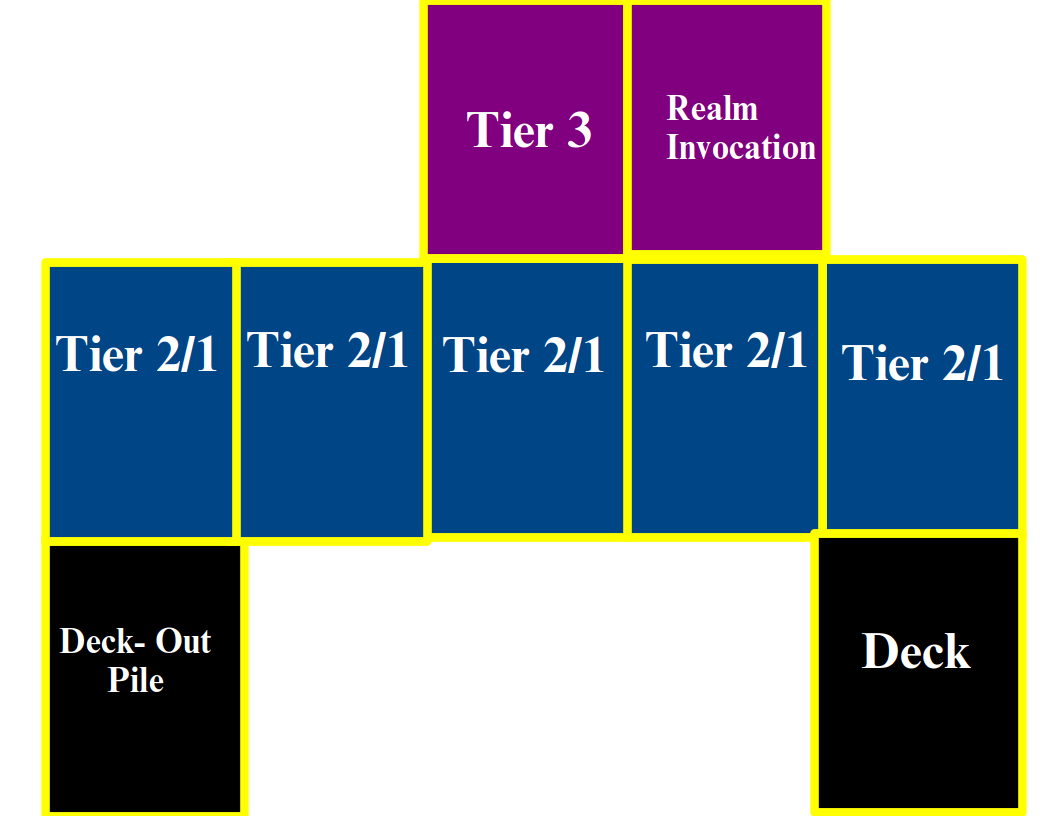
\includegraphics[scale=0.22]{images/field.png}
        \caption{\textrm{Layout of Battlefield}}
    \end{figure}
\end{frame}

\begin{frame}
    \frametitle{Explaining Layout}

    

\end{frame}



\begin{frame}
    \frametitle{Phases}
    %
    \textrm{While playing Phaktionz there are 5 phases during a turn, the phases go as follows:} 
    %
    \begin{alertblock}{Draw Phase}
        \textrm{The Player begins their turn by a drawing a card from their deck}
    \end{alertblock}
    %
    \begin{alertblock}{Main Phase}
       \textrm{The Player can now place their summons or activate their invocations}
    \end{alertblock}
    %
    \begin{alertblock}{Combat Phase}
        \textrm{The Player can now battle different summons on the opposing battlefield}
    \end{alertblock}

\end{frame}




%--------------------------------------------------
\section{Single Player vs Multi-Player}





%--------------------------------------------------
\section{Formats}
\end{document}